\chapter{Hazel Bugs: Unboxing}
\label{sec:UnboxingBugs}
When a final form (\cref{sec:HazelFinalForms}) has a type, Hazel often needs to extract parts of the term according to the type during evaluation.

For example, if a term is a final form of type list, then it could be either:
\begin{itemize}
\item A list literal: \code{[1,2,3]}.
\item A list with casts wrapped around it: \code{[1,2,3]}$\scast{\code{[Int]}}{\code{[}\dyn\code{]}}$.
\item A list cons with indeterminate tail: \code{1::2::?}.
\end{itemize}
Additionally, when the input is not a list at all, it returns \code{DoesNotMatch}, used in pattern matching.  Unboxing makes use of GADTs to allow for varying output type depending on the type that the final form is being unboxed upon.

\subsubsection{Hazel Unboxing Bugs}
While writing the search procedure I found various unboxing bugs in Hazel. Programs exhibiting these were removed from the evaluation data, whereas some bugs were fixed by myself (hence, not removing from the evaluation data). 

For example, there was the following bug, affecting pattern matching. A list cons which has an indeterminate tail would \textit{indeterminately match} with \textit{any} list literal pattern (of \textit{any} length), even when it is known for certain that it could never match. For example a list cons \code{1::2::?} represents lists with length $\geq 2$, but even when matching a list literal of length 0 or 1 it would indeterminately match rather than explicitly \textit{not} match. 

Pattern matching checks if each pattern matches the scrutinee with the following behaviour, starting from the first branch:
\begin{itemize}
\item \textit{Branch matches?} Execute the branch.
\item \textit{Branch does not match?} Try the next branch.
\item \textit{Branch indeterminately matches?} Cannot assume the branch doesn't match so must stop evaluation here. The match statement is then indeterminate.
\end{itemize}
\Cref{fig:PatternMatchingBug} demonstrates a concrete example which would get stuck in Hazel, but does \textit{not} need to. I reported and fixed this, with my PR merged into the dev branch.

\begin{figure}[H]
\centering
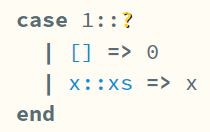
\includegraphics[width=0.25\textwidth]{Media/Figures/unboxing_bug}
\caption{Pattern Matching Bug}
\label{fig:PatternMatchingBug}
\end{figure}
